\subsection{Мобильная разработка}
Конечный успех программного проекта во многом определяется до начала конструирования: на этапе подготовки, которая проводится с учетом всех особенностей проекта.

Первое предварительное условие, которое нужно выполнить перед конструированием, -- ясное формулирование проблемы, которую система должна решать. Общая цель подготовки — снижение риска: адекватное планирование позволяет исключить главные аспекты риска на самых ранних стадиях работы, чтобы основную часть проекта можно было выполнить максимально эффективно. 

Главный факторы риска в создании ПО — неудачная выработка требований. Требования подробно описывают, что должна делать программная система. Внимание к требованиям помогает свести к минимуму изменения системы после начала разработки \cite{code_complete}.

Перед формулированием требований необходимо изучить ряд вопросов, которые напрямую влияют на все дальнейшие этапы разработки. В частности, необходимо рассмотреть вопросы выбора платформ, архитектуры. По результатам анализа можно будет составить техническое задание к проектируемому программному средству, которое станет основой для составления функциональных требований.

\subsubsection{}
\label{sec:analysis:literature:platforms}

Разработка мобильных приложений, становится все более и более
востребованной, таким образом разработчики ищут новые возможности для
быстрой и качественной реализации проектов. Долгое время разработка
мобильных приложений являлась исключительно нативной, это обусловлено
достаточным качеством и быстродействием существующих IDE.

Таким образом, для того, что бы написать качественные программы для
двух наиболее распространенных платформ (Android, IOS) необходимо было
изучать такие языки программирования, как: Java, Kotlin, Swift~\cite{swift}, ObjectiveC~\cite{objectiveC}. Благодаря необходимости знания множества языков, компанией
Facebook был представлен фреймворк ReactNative~\cite{reactNaitve}, для написания на
котором требовалось знание JavaScript.

В ReactNative, в качестве ЯП используется
JavaScript, или несколько иной подход смешивающий синтаксис JavasScript и
HTML по типу JSX. Инструменты для ReactNative – это в основном текстовый
редактор, отладчик Chrome и несколько других инструментов для сборки и
тестирования. 

Для нативной разработки IOS необходимо знание языка Swift или
Objective-C, а для Android – Java или Kotlin. Инструменты для создания
приложения находятся в IDE каждой платформы: для IOS это X-code, а для
Android это Android studio. Так же для программирования в каждой из этих IDE,
необходимо знать как работать в этой среде, как работают системы отладки и
сборки.

ReactNative берет свое начало в веб-разработке и заимствует свою
базовую части именно оттуда, в то время как для нативной разработки такой
базовой части не существует. Это исключительно нативные сенсорные
платформы, которые необходимо изучать. Так же стоит отметить, что когда
изучена одна из IDE, вторая изучается достаточно быстро.

Фреймворки являются очень значимым показателем выбора в сторону
нативной разработки. Необходимо изучить как работают все интересующие вас
функции, но в отличии от ReactNative, все эти функции задокументированы и
реализованы. 

\begin{figure}[H]
	\centering
	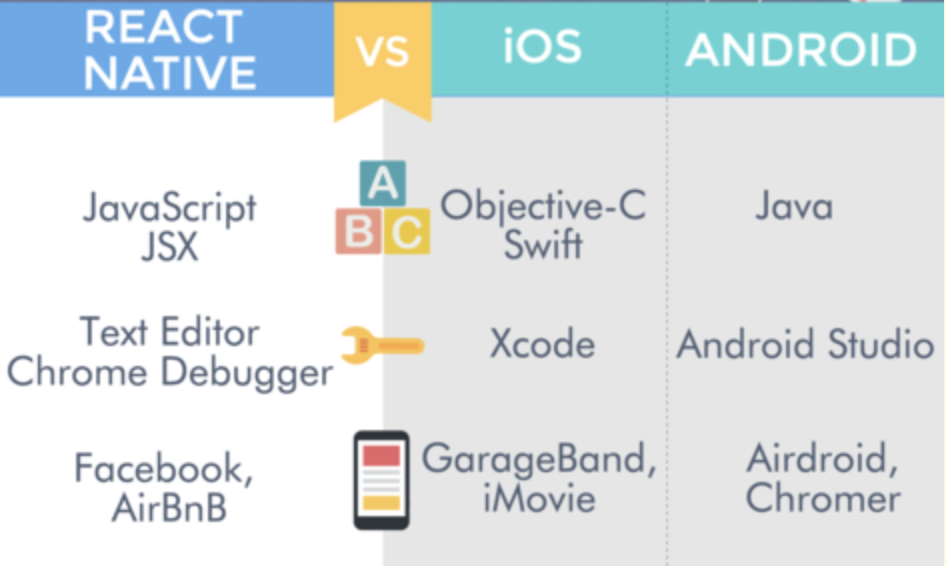
\includegraphics[scale=1]{rn-vs-androi-vsios.png} 
	\caption{Сравнение нативной и кроссплатформенной разработки}
	\label{fig:analysis:analogues:bsuir}
\end{figure}

Swift и ReactNative совсем недавно появились в программировании, при
этом каждый из них отлично документирован. Официальная документация
apple, позволяет разобраться во всех тонкостях нового языка, с примерами
применения и полезными советами начинающим разработчикам. В то же время 
официальная документация Facebook по ReactNative, тоже раскрывает все
возможности фреймворка, с примерами кода и типовой документацией. 

\subsubsection{}
\label{sec:analysis:literature:architecture}

Существует множество различных архитектурных шаблонов для
разработки мобильных IOS приложений. Выбор архитектуры будущего
приложения очень важный этап проектирования. Правильный выбор
архитектуры, позволит проводить поиск ошибок, а так же оперативно
реагировать на изменения внутри класса. 

В настоящее время есть множество вариантов шаблонов проектирования
архитектуры, среди них выделяются следующие: MVC, MVP, VIPER.
MVC, MVP, MVVM предполагают включение объектов приложения в
одну из трех категорий: 
\begin{itemize}
	\item Models -- ответственные за данные домена или уровень доступа к
	данным, который манипулирует данными;
	\item Views -- ответственны за уровень представления, все элементы с префиксом UI;
	\item Controller, Presenter, ViewModel -- выполняет роль посредника
	между Model и View, отвечающего за изменения Model и реагируя на действия
	пользователя, выполняемые во View и обновляя View с изменениями из Model.
\end{itemize}

Далее подробнее рассмотрим каждый из представленных выше
шаблонов.

При использовании шаблона традиционного MVC, View не имеет
состояния, он просто отображается контроллером после изменения модели~\cite{mvc}.
Таким образом, этот шаблон подразумевает полную перезагрузку страницы
после любого действия пользователя.

Таким образом, реализация традиционного MVC в приложении IOS не
имеет смысла из-за архитектурной проблемы – все три объекта связаны друг с
другом и каждая сущность знает о двух других (рисунок~\ref{fig:analysis:tradMvc}).

\begin{figure}[H]
	\centering
	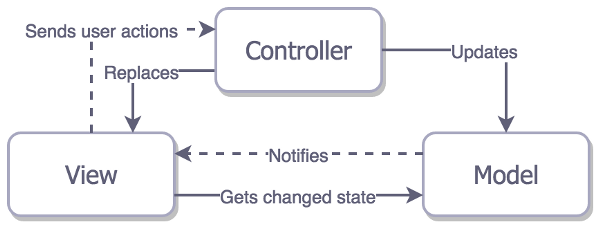
\includegraphics[scale=0.55]{traditionalMVC.png} 
	\caption{Традиционный MVC}
	\label{fig:analysis:tradMvc}
\end{figure}

В шаблоне архитектуры Apple MVC (рисунок~\ref{fig:analysis:appleMVC}) контроллер будет являться
посредником между View и Model, что бы эти два объекта не знали о
существовании друг друга~\cite{mvcApple}. Наиболее часто используемым объектом будет
являться контроллер. В этом есть плюсы, потому что в приложении должно
быть место для всей сложной бизнес-логики, которая не вписывается в Model. 

\begin{figure}[H]
	\centering
	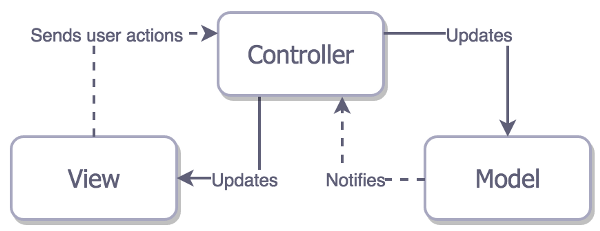
\includegraphics[scale=0.55]{appleMVC.png} 
	\caption{Apple MVC}
	\label{fig:analysis:appleMVC}
\end{figure}

В реальности шаблон Apple MVC работает по-другому.
Перегруженный контроллер содержит в себе большое количество бизнеслогики, превращая Model-View-Controller в Massive-View-Controller. Cocoa
MVC поощряет писать Massive-View-Controller, потому что они вовлечены в жизненный цикл View, что приводит к неразделимости
этих двух сущностей (рисунок~\ref{fig:analysis:realAppleMVC}). 

\begin{figure}[H]
	\centering
	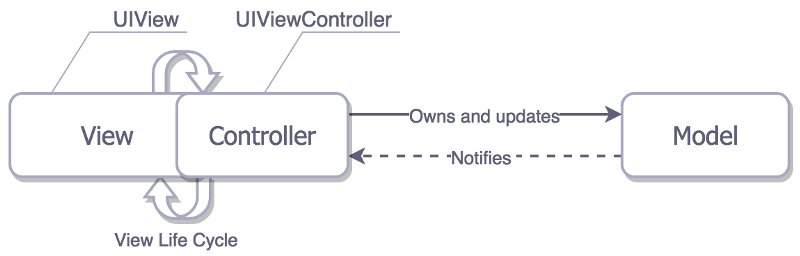
\includegraphics[scale=0.55]{realAppleMVC.png} 
	\caption{Практический Apple MVC}
	\label{fig:analysis:realAppleMVC}
\end{figure}

MVP (Cocoa MVC’s promises delivered) похож на Apple MVC, но это не
так[16]. В Apple MVC – View связан с контроллером, в то время как медиатор
MVP – Presenter, не имеет ничего общего с жизненным циклом контроллера,
поэтому в Presenter нет кода для установки макета экрана, но он отвечает за
обновление View с актуальными данными и состоянием. 

MVP это архитектурный шаблон, показывающий проблемы сборки,
которая возникает из-за наличия трех фактически разделенных слоев (рисунок~\ref{fig:analysis:mvpPic}).

\begin{figure}[H]
	\centering
	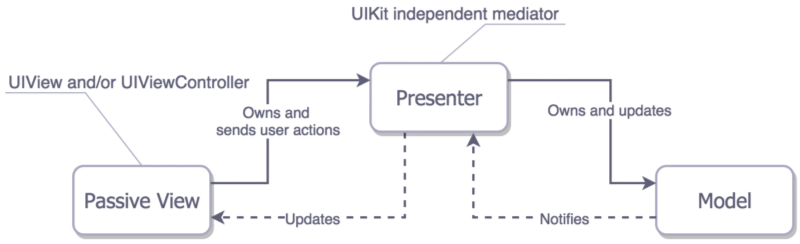
\includegraphics[scale=0.55]{mvp.png} 
	\caption{MVP}
	\label{fig:analysis:mvpPic}
\end{figure}

Существует и другой формат MVP – MVP Supervising Controller~\cite{mvcAppleReal}.
Этот вариант включает прямую зависимость View и Model, в то время как
Presenter (Supervising Controller) все еще обрабатывает действия из View и
способен его изменять. Разделение смутной ответственности, является
недопустимым, так же как и сильная связь View и Model (рисунок~\ref{fig:analysis:MvPbh}). 

\begin{figure}[H]
	\centering
	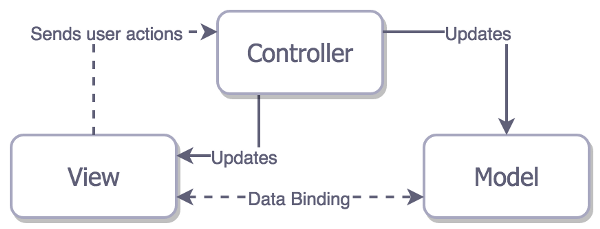
\includegraphics[scale=0.55]{MvPbh.png} 
	\caption{MVP (Bindings and Hooters)}
	\label{fig:analysis:MvPbh}
\end{figure}

MVVM рассматривает контроллер View, как View, а так же
подразумевает отсутствие связи между View и Model~\cite{mvvmApple}. View-Model
обеспечивает независимое представление View и его состояния. View-Model
вызывает изменения в Model и обновляет себя с обновленной Model, а
поскольку View и View-Model соединены, View соответственно тоже
обновляется (рисунок~\ref{fig:analysis:mvvm}). 

\begin{figure}[H]
	\centering
	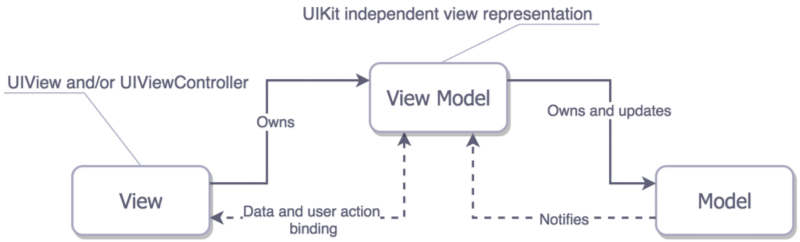
\includegraphics[scale=0.55]{mvvm.png} 
	\caption{MVVM}
	\label{fig:analysis:mvvm}
\end{figure}

VIPER позволяет полностью разделить обязанности, и обеспечить
полную независимость модулей~\cite{viper}. Он состоит из: 
\begin{itemize}
	\item View – отвечающее за исполнение произошедших в Presenter
	изменений;
	\item Presenter – содержит связанную с UI (независимую от UIKit)
	бизнес-логику, вызывает методы в Interactor;
	\item Entities – в этом классе хранятся простые объекты данных;
	\item Interactor – содержит бизнес-логику, связанную с данными
	(Entities) или сетевыми устройствами. В его обязанности входят такие
	операции, как создание новых экземпляров объектов, или выборку их с сервера.
	Для этих целей используются службы и менеджеры, не являющиеся частью
	модуля VIPER – они являются внешней зависимостью (рисунок~\ref{fig:analysis:viper}).
\end{itemize}

\begin{figure}[H]
	\centering
	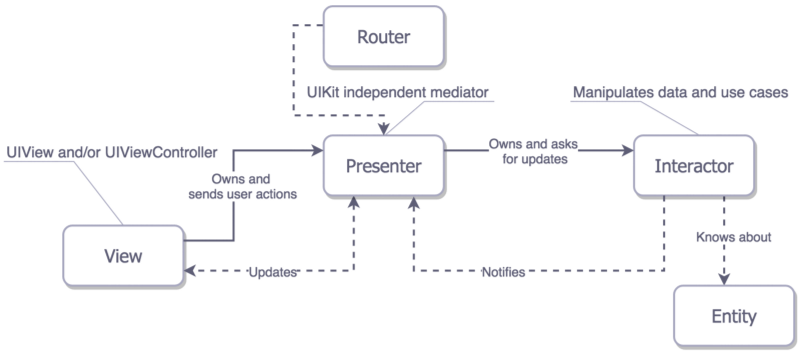
\includegraphics[scale=0.55]{viper.png} 
	\caption{VIPER}
	\label{fig:analysis:viper}
\end{figure}

Модуль VIPER может соответствовать как одному экрану в
приложении, так и всему приложению, четких указаний как выбрать размер
модуля не приводится.
VIPER – это первый шаблон в котором явно рассматривается
навигационная ответственность, которая решается при помощи Router.

% \subsubsection{} Проектирование баз данных
% \label{sec:analysis:literature:db}

% В настоящее время сложно представить сложные приложения, которые бы не использовали специальные средства для хранения информации.

% База данных -- представленная в объективной форме совокупность самостоятельных материалов, систематизированных таким образом, чтобы эти материалы могли быть найдены и обработаны с помощью ЭВМ. Модель базы данных -- описание базы данных с помощью  определенного (в т.ч. графического) языка на некотором уровне абстракции.


